\def\year{2018}\relax
%File: formatting-instruction.tex
\documentclass[letterpaper]{article} %DO NOT CHANGE THIS
\usepackage{aaai18}  %Required
\usepackage{times}   %Required
\usepackage{helvet}  %Required
\usepackage{courier} %Required
\usepackage{url}     %Required
\usepackage{graphicx}%Required
\usepackage{color}
\usepackage{algorithm}
\usepackage{algorithmic}
\usepackage{diagbox}
\usepackage{multicol,multirow}
\usepackage[tight,footnotesize]{subfigure}

\nocopyright

\frenchspacing  %Required
\setlength{\pdfpagewidth}{8.5in}  %Required
\setlength{\pdfpageheight}{11in}  %Required

\graphicspath{{./Imgs/}}
\DeclareGraphicsExtensions{.pdf,.jpg,.png}
\newcommand{\figref}[1]{Fig.~\ref{#1}}
\newcommand{\tabref}[1]{Tab.~\ref{#1}}
\newcommand{\secref}[1]{Sec.~\ref{#1}}
\newcommand{\algref}[1]{Algorithm~\ref{#1}}
\newcommand{\equref}[1]{Equ. (\ref{#1})}
\newcommand{\parahead}[1]{\textbf{#1}}
\newcommand{\myPara}[1]{\vspace{.1in}\textbf{#1}}
\def\ie{\emph{i.e.~}}
\def\eg{\emph{e.g.~}}
\def\etc{\emph{etc}}
\def\vs{\emph{vs.~}}
\def\etal{{\em et al.~}}
\def\sArt{{state-of-the-art~}}
\newcommand{\todo}[1]{{\textcolor{red}{#1}}}
\newcommand{\cmm}[1]{{\textcolor{blue}{#1}}}

%PDF Info Is Required:
\pdfinfo{
/Title (RefinedBox: Towards Object Proposal Refinement and Joint Object Detection)
/Author (AAAI Press Staff)}

\setcounter{secnumdepth}{0}

\begin{document}
%
\title{RefinedBox: Towards Object Proposal Refinement and Joint Object Detection}
\author{Anonymous AAAI submission\\
Paper ID 125\\
% \author{Yun Liu, Ming-Ming Cheng, Shi-Jie Li, Peng-Tao Jiang, JiaWang Bian\\
% College of Computer and Control Engineering, Nankai University\\
% Tianjin, China\\
}
\maketitle


%%%%%%%%%%%%%%%%%%%%%%%%%%%%%%%%%%%%%%%%%%%%%%%%%%%%%%%%%%%%%%%%%%%%%%%%%%%%%%%
\begin{abstract}
Object detection is a fundamental and widely used computer vision technique.
Recently, object proposal generation has shown value for object
detection by hypothesizing object locations.
High-quality object proposals that provide highly accurate but relatively
few candidates would greatly benefit object detection.
We note that many bottom-up proposal methods generate dense proposals
to cover as many objects as possible but that (i) they usually fail to rank these
proposals properly and (ii) the number of proposals is very large.
In this paper, we design a computationally lightweight neural network to refine
the initial object proposals.
The proposed network can share convolutional layers with object detection by
joint training, so the proposal refinement is very fast.
Extensive experiments demonstrate that our method can produce \sArt object
proposals compared with the well-known proposal generation methods such
as RPN, Selective Search, and Edge Boxes.
The proposed object detection method also performs better than Faster R-CNN.
\end{abstract}


%%%%%%%%%%%%%%%%%%%%%%%%%%%%%%%%%%%%%%%%%%%%%%%%%%%%%%%%%%%%%%%%%%%%%%%%%%%%%%%
\section {Introduction}
%
In the past few years, convolutional neural networks have driven a number of
recent advances in object detection.
% object detection has undergone a great development due to
% the success of convolutional neural network.
%
The \sArt object detection methods can be grouped into two main classes:
region-free methods \cite{redmon2016you,liu2016ssd}
and region-based methods \cite{girshick2014rich,girshick2015fast,ren2015faster}.
%
The region-free methods seek to detect and recognize objects directly from natural images.
This category of methods is very efficient while suffering the decline of accuracy.
%
The region-based methods have shown high accuracy on mainstream object detection
benchmarks \cite{lin2014microsoft,pascal-voc-2007}.
These methods usually produce object proposals first and then
train deep models to classify these proposals.
Thus proposal generation is very important for object detection because it provides
the search space for follow-up classification.


\begin{figure}[t]
	\centering
    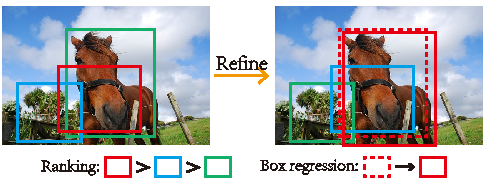
\includegraphics[width=\linewidth]{box_refinement}
    \caption{The overview of object proposal refinement.The left image shows the
    	original proposals, and the right image shows the results after refinement.
        We first re-rank the proposals by computing new objectness scores, after
        which a box regression procedure is applied to each proposal box for
        accurate location.}
    \label{fig:refinement_overview}
\end{figure}


%Since object proposals will \cmm{usually} be fed into object detection framework later,
%a good proposal method should produce a small number of proposals while
%covering as many objects in an image as possible.
Generating \emph{a small number of} object proposals while covering as
many objects in an image as possible is crucial for the efficiency
and accuracy of object detection systems,
by reducing the search space and false alarms.
%
Many object proposal methods have been developed such as Selective Search
\cite{uijlings2013selective}, Edge Boxes \cite{zitnick2014edge} and
MCG \cite{arbelaez2014multiscale}.
%
Recently, RPN \cite{ren2015faster}, a deep learning based proposal
method, has attracted a lot of attention in this field because it can provide
high detection recall with much fewer candidate boxes.
However, the number of true objects (\eg usually less than 10)
is still much smaller than the RPN proposals (\eg a few hundred).
%
Can we significantly reduce the number of proposals while maintaining
high recall?
This is not only useful for further improving the object detection systems,
but also crucial for a much wider range of applications,
\eg mining knowledge from huge amount of unlabeled/weakly-labeled 
data \cite{wei2016hcp,wu2015deep},
for which the large number of false positives will pose significant challenges
not only for computational efficiency but also for system stability.

%The small number of proposals is not only necessary for the efficiency
%of follow-up detection, but also necessary for the detection accuracy
%by reducing the false alarms.
%Usually, only several hundred proposals of RPN are sufficient to cover most
%of the objects in an image.
%%
%Can the quality of object proposals be further improved?
%The answer is yes.


We observe that some proposal generation methods can achieve high detection
recall when the number of candidate boxes is sufficiently large.
The large number of candidates of course causes many false positives in
the subsequent detection and thus affects the detection accuracy.
%
However, if we can select the good ones from the large set of candidates,
higher detection performance may be achieved.
%
Several algorithms have been proposed to refine object proposals,
including DeepBox \cite{kuo2015deepbox} and MTSE \cite{chen2015improving}.
DeepBox builds a neural network to recompute the objectness scores of the
initial boxes and then re-rank them.
MTSE tries to refine each box using superpixels by making each box tightly
cover some inner superpixels.
However, DeepBox has to build a separate neural network, and the quality of
generated proposals is worse than RPN.
The performance of MTSE depends on the quality of superpixels,
and the image segmentation within MTSE causes a significant increase in
computational load.


In this paper, we propose a novel method to re-rank and align existing proposal
boxes in a single inference of a neural network.
An overview of our approach is shown in \figref{fig:refinement_overview}.
Our refinement of candidate boxes includes two steps: re-ranking and box regression.
The re-ranking step tries to re-rank the proposals according to the
tightness of their coverage with complete objects.
The box regression step attempts to fine tune the shapes and locations of boxes
in order to make them cover real objects more tightly.
%
To achieve this goal, our refinement network is designed to learn new objectness
scores and perform box regression simultaneously.
The proposed network is also computationally lightweight,
so it can be applied in detection algorithms with a little extra time consumption.
The training process of refinement can be performed in an end-to-end manner.
%
For the sake of brevity, we call our proposed method \textbf{RefinedBox} in the
remainder of this paper.
%
To unify RefinedBox and the well-known Fast R-CNN \cite{girshick2015fast}
detection framework, we connect our refinement layers after the last convolutional
layer of the base network such as VGG16 \cite{simonyan2014very}.
We follow the alternating fine-tuning training used in Faster R-CNN.
As a result, our refinement network can share the base convolutional layers with
the consequent object detection network, making the refinement procedure very efficient.


Using the proposal boxes produced by Edge Boxes \cite{zitnick2014edge} as input,
we train and test our network on the VOC2007 dataset \cite{pascal-voc-2007} using VGG16.
For object proposal generation, our method achieves the detection recall of
97.8\% and 91.7\% for intersection-over-union (IoU) 0.5 and 0.7,
respectively, using 300 refined boxes per image.
For object detection, our method achieves a mean average precision (mAP) of
71.1\% compared with the mAP of 69.2\% for Faster R-CNN \cite{ren2015faster}.
Thus, our proposed RefinedBox method can generate more accurate object proposals
than RPN which is used in Faster R-CNN.
The code of this paper will be published as soon as the paper is accepted.



%%%%%%%%%%%%%%%%%%%%%%%%%%%%%%%%%%%%%%%%%%%%%%%%%%%%%%%%%%%%%%%%%%%%%%%%%%%%%%%
\section{Related Work}
%
Since this paper is mainly about object proposal refinement,
we first briefly describe recent developments in object detection.
We then go on to discuss object proposal generation.
We broadly divide the related research on object proposal generation
into three parts: segmentation-based methods,
edge-based methods, and proposal post-processing methods.


\myPara{Object detection} is a fundamental and widely used technique
in computer vision.
Object detection aims to detect all objects of interest in an image
and recognize their categories.
%
With the great success of the convolutional neural networks (CNNs) on large
scale object recognition tasks in recent years, more and more methods based
on CNNs have been proposed \cite{girshick2014rich,girshick2015fast}.
These object detection methods can be broadly divided into two groups:
region-based methods and region-free methods.
%
The region-based methods divide this task into two steps of object proposal
generation and the post-classification of these proposals.
R-CNN \cite{girshick2014rich} is the first method that uses semantic information
in neural networks to classify object proposals.
Then, some of its variants were proposed, including
SPPNet \cite{he2014spatial}, Fast R-CNN \cite{girshick2015fast},
and Faster R-CNN \cite{ren2015faster}.
%
The region-free methods \cite{liu2016ssd,redmon2016you,redmon2016yolo9000}
skip the region proposal step and directly predict the location and category
for each object.
This kind of methods is very efficient with the sacrifice in detection accuracy.


\myPara{Segmentation-based object proposal generation methods}
use the image segmentation as input and try to find the proper combinations
of these image segments to cover all complete objects.
These methods usually combine some low-level features (such as saliency, color,
SIFT \etal) to score the bounding boxes and then select boxes with high scores.
%
For example, Selective Search \cite{uijlings2013selective}, one of the most popular
object proposal methods, uses the strength of exhaustive search and segmentation to
obtain high-quality proposals by a hierarchical merging of superpixels.
%
\cite{arbelaez2014multiscale,rahtu2011learning,endres2014category,manen2013prime,rantalankila2014generating,krahenbuhl2015learning} also fall into this category.


\myPara{Edge-based proposal methods} exploit the observation that complete objects
in natural images usually have well-defined closed boundaries \cite{alexe2012measuring}.
In recent years, several efficient algorithms have been proposed using the edge feature.
Zhang \etal \cite{zhang2016object} designed a cascaded ranking SVM (CSVM) method
to obtain proposals using gradient features.
\cite{cheng2014bing} proposed a very efficient algorithm, BING, which
runs at 300 fps by quantizing \cite{zhang2016object} into some binary operations.
Edge Boxes \cite{zitnick2014edge} computes the objectness scores according to
the number of contours that are wholly contained in each bounding box.


\begin{figure*}[t]
	\centering
    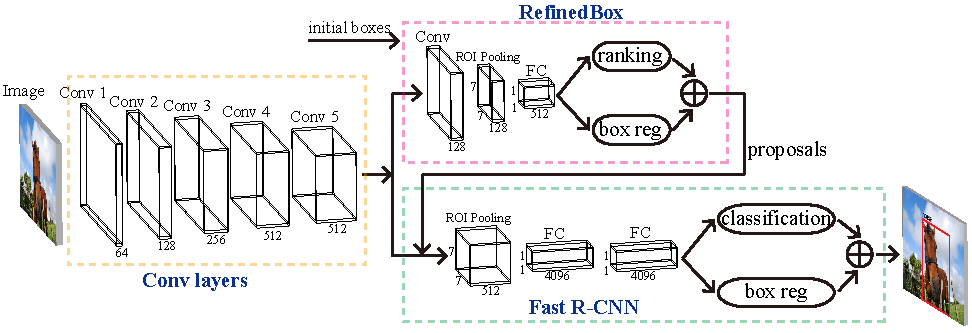
\includegraphics[width=\linewidth]{network}
    \caption{The overview of our network architecture. The proposed network takes a
    	nature image and corresponding initial boxes produced by other object proposal
        generation methods such as Edge Boxes as input. The branch of RefinedBox is
        designed to refine the initial boxes, then the refined boxes are inputted into
        the branch of Fast R-CNN for classification. Note that the refinement of boxes
        and consequent object detection can share the convolutional features.}
    \label{fig:network}
\end{figure*}


\myPara{Proposal post-processing} aims to refine the object proposals in
order to accurately locate objects in an image.
%
Kuo \etal \cite{kuo2015deepbox} proposed a small neural network called DeepBox
to recompute the objectness scores of the existing boxes and then re-rank these
boxes according to the new objectness scores.
%
Chen \etal \cite{chen2015improving} tried to align the proposal boxes with the
superpixels.
%
Zhang \etal \cite{zhang2017sequential} further discussed the optimization of
object proposal generation.
They first used edges and then superpixels to optimize the proposal boxes.
Their segmentation based optimization accelerates the superpixel generation in MTSE
\cite{chen2015improving}, thus the resulting system can be run at a very fast speed.
%
\cite{he2015oriented} proposed oriented object proposals that have different
orientations, not only the vertical boxes used in regular methods.
%
In this paper, we build a refinement network that can share the convolutional layers
with subsequent classification for object detection.
The refined boxes produced by our method achieve the \sArt performance both for
object proposal generation evaluation and object detection evaluation.



%%%%%%%%%%%%%%%%%%%%%%%%%%%%%%%%%%%%%%%%%%%%%%%%%%%%%%%%%%%%%%%%%%%%%%%%%%%%%%%
\section{RefinedBox}
%
\subsection{Network Architecture}
%
Our method takes the object proposals produced by other proposal generation methods
as input and then tries to refine them.
The refinement includes twofold: re-ranking and box regression.
To re-rank the existing boxes, we recompute the objectness score for each box
using the semantic information in the deep neural network.
To obtain the box regression, the network is designed to learn the regressions
of the center coordinates, width, and height for each box.


VGG16 \cite{simonyan2014very} is a widely used base network architecture
in deep learning research.
It is composed of 13 convolutional layers and 3 fully connected layers.
Inspired by previous literature \cite{girshick2015fast,ren2015faster},
we build our network based on VGG16 to showcase our refinement method.
Our network architecture is shown in \figref{fig:network}.
Our network takes a natural image and corresponding initial boxes as input.
The initial boxes are produced by other object proposal generation methods.
In this paper, we use some well-known proposal generation methods as examples.
The input image first undergoes a forward pass through some convolutional layers,
\eg the 13 convolutional layers in VGG16.
In order to reduce the time consumption of box refinement,
we design a computationally lightweight neural network.
Thus, we first connect a convolutional layer with kernel size $3 \times 3$ after
the \textit{Conv 5} layer to reduce the number of channels from 512 to 128.
Then, a \textit{ROI Pooling} layer is followed to down-sample each initial box region
into a fixed feature map size, \ie $7 \times 7$.
Next, a fully connected layer with only 512 output neurons is connected.
At last, two branches of scoring and box regression are used to recompute the
objectness score and obtain the location offsets of each initial box.
In addition, a ReLU layer is followed after the added \textit{Conv} layer
and \textit{FC} layer, respectively.


For training RefinedBox, each initial box is assigned a binary class label of being
an object or not.
The loss function can be written as
\begin{equation}
L_{obj}(p,u) = -[1_{\{u=1\}}log~p_1 + 1_{\{u \neq 1\}}log~p_0],
\end{equation}
where $p$ is computed by a softmax over the two outputs of a fully connected layer
and $u$ is the label of this box (1 or 0).
The box regression layer is a fully connected layer which is designed to learn
the coordinate offsets.
We follow \cite{girshick2014rich} to perform the parameterizations of four coordinates:
two coordinates of box center, width, and height.
Thus the joint loss function can be written as
\begin{equation}
L(p,u,t,v) = L_{obj}(p,u) + \lambda \cdot 1_{\{u=1\}} L_{reg}(t,v),
\end{equation}
where $v$ is the regression target and $t$ is the predicted tuple.
The parameter $\lambda$ is a balance parameter, and we set it as 1 in this paper.
We use the regression loss in \cite{girshick2015fast} to compute $L_{reg}$.


Each SGD mini-batch is constructed from an image in which 256 boxes are selected
as training samples.
In each batch, half of the sampling boxes are positive samples and the other half
are negative.
These positive samples have IoU overlap with a ground truth box of at least 0.7,
while the negative samples are boxes whose max IoU overlap with ground truth
is in the interval [0.1, 0.5).
The initial learning rate is set to 1e-3 and will be divided by 10 after
60k iterations.
We run SGD for 80k iterations in total.


\begin{algorithm}[tb]
\begin{algorithmic}
	\STATE \textbf{Step 1:} Initialize the proposal module with the model pre-trained
    	on ImageNet, and fine-turn the proposal module.
    \STATE \textbf{Step 2:} Re-rank the initial proposals using the trained model in
    	\textbf{Step 1}.
    \STATE \textbf{Step 3:} Fine-turn the detection module using the re-ranked proposals,
    	initializing from pre-trained ImageNet model.
    \STATE \textbf{Step 4:} Initialize from the detection model in \textbf{Step 3},
    	but keep the shared convolutional layers fixed and only fine-turn the unique
        layers to RefinedBox.
    \STATE \textbf{Step 5:} Re-rank the initial proposals using the trained model in
    	\textbf{Step 4}.
    \STATE \textbf{Step 6:} Keep the shared convolutional layers fixed and only
    	fine-turn the \textit{FC} of the Fast R-CNN.
\end{algorithmic}
\caption{Alternative fine-turning of RefinedBox.}
\label{alg:training}
\end{algorithm}


\begin{figure*}[!ht]
  \centering
  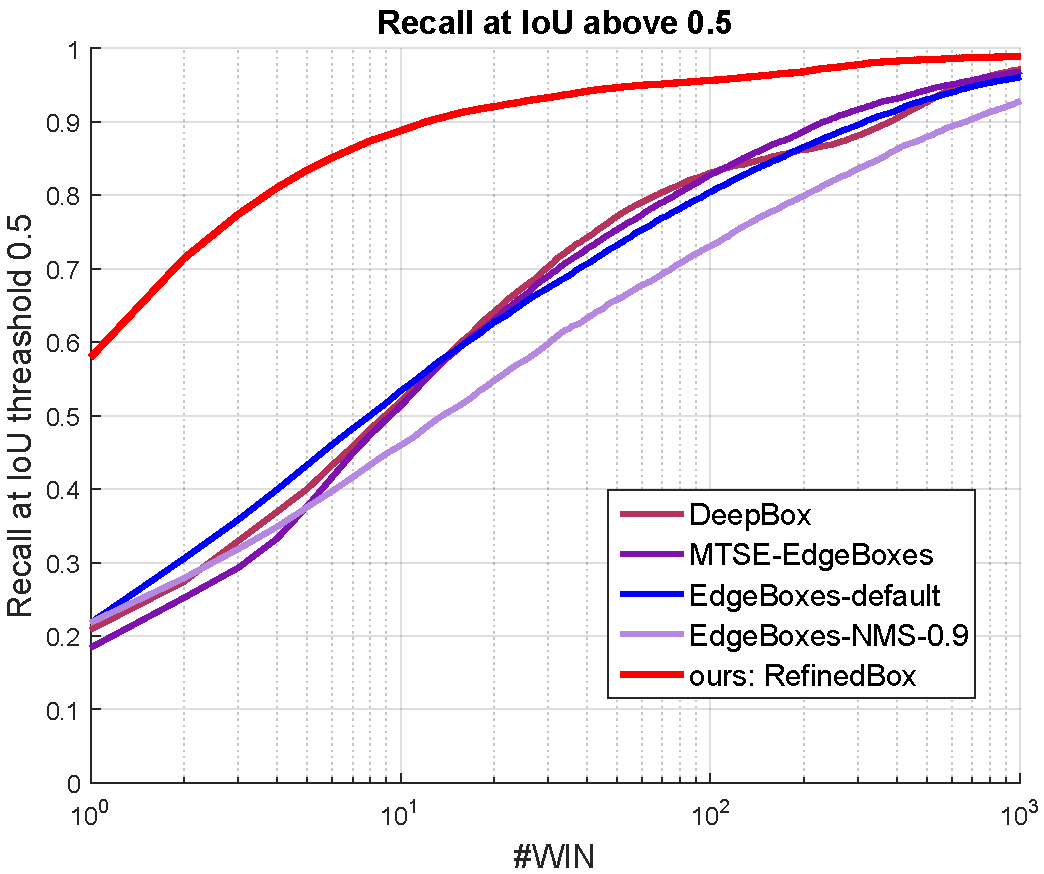
\includegraphics[width=.425\linewidth]{refine-recall-proposals-0_5} \hspace{.03\linewidth}
  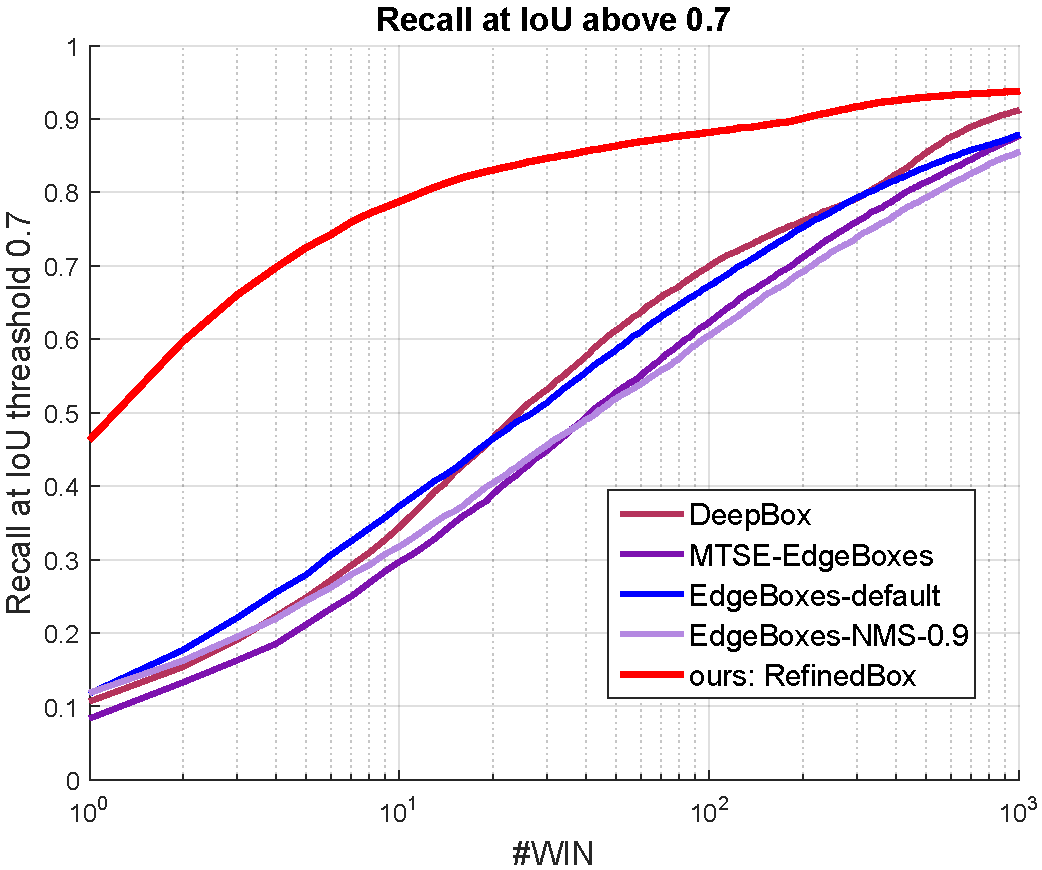
\includegraphics[width=.425\linewidth]{refine-recall-proposals-0_7} \\
  \caption{The evaluation of different refinement algorithms. These two subfigures
  	show object detection recall \vs the number of proposals (\#WIN) at IoU threshold
    0.5 (left) and 0.7 (right) respectively. The method of EdgeBoxes-default is
    the Edge Boxes \cite{zitnick2014edge} using default parameters, and the
    EdgeBoxes-NMS-0.9 changes the parameter of non-maximum suppression (NMS)
    to 0.9.}
  \label{fig:refine-evaluation}
\end{figure*}


\subsection{Joint Training with Object Detection} \label{sec: detection}
%
So far we have described how to train the proposal refinement network,
and now we focus on the joint object detection task.
%
As shown in \figref{fig:network}, we connect the well-known detection framework,
Fast R-CNN \cite{girshick2015fast}, after the convolutional layers as a parallel
branch to RefinedBox.
The refined proposals produced by the RefinedBox branch are inputted into Fast R-CNN.
%
In order to make the RefinedBox and Fast R-CNN share the same convolutional features,
we apply an alternating fine-turning process.
The algorithm is presented in \algref{alg:training}.
After the alternating training, both networks form a unified network.
%
For each proposal box, there are 120.0 million FLOPs for the fully connected layers
of the Fast R-CNN branch, while only 3.2 million FLOPs for the fully connected layers
of the RefinedBox branch.
Thus, the RefinedBox branch only incurs a little extra computational load.


For training the detection module, each mini-batch has 256 object proposals that
are from the same image.
As in Fast R-CNN, 25\% of these proposals have IoU overlap with a ground truth
of at least 0.5, and they are viewed as positive samples.
The remaining negative samples have max IoU overlap with ground truth
in the interval [0.1, 0.5).
The top 2000 proposals generated by RefinedBox are used in training.
The learning rate is 1e-3 for the first 50k iterations of SGD,
and then the learning rate is divided by 10 for another 20k iterations.
For testing, the top 300 proposals (per image) of RefinedBox are used.
In contrast, the traditional proposal methods, such as Edge Boxes and
Selective Search, need thousands of proposals.



%%%%%%%%%%%%%%%%%%%%%%%%%%%%%%%%%%%%%%%%%%%%%%%%%%%%%%%%%%%%%%%%%%%%%%%%%%%%%%%
\section{Experiments}
%due to space constraints.
We evaluate our method on the widely used PASCAL VOC2007 dataset
\cite{pascal-voc-2007} which is composed of 2501 training, 2510 validation, and
4952 test images with corresponding annotations across 20 object categories.
All the experiments in this paper are trained on the VOC2007 \textit{trainval}
set and tested on the VOC2007 \textit{test} set.
% The input can also be replaced by other proposal
% generation methods since our method is generic for box refinement.
The experiments are conducted on a GTX TITAN X GPU using the publicly
available code \footnote{https://github.com/rbgirshick/py-faster-rcnn}.


Our experiments are divided into two parts.
The first part contains the comparison about object proposal, in which we
compare the existing mainstream proposal methods with ours in detail.
In the second part, we feed the proposals produced by these methods into a
region-based object detection framework, Fast R-CNN \cite{girshick2015fast},
to evaluate the quality of proposals in object detection.
Our experiments demonstrate that our method can generate high-quality
proposals for object detection with good efficiency.


\begin{figure*}[!htbp]
  \centering
  \subfigure[]{
  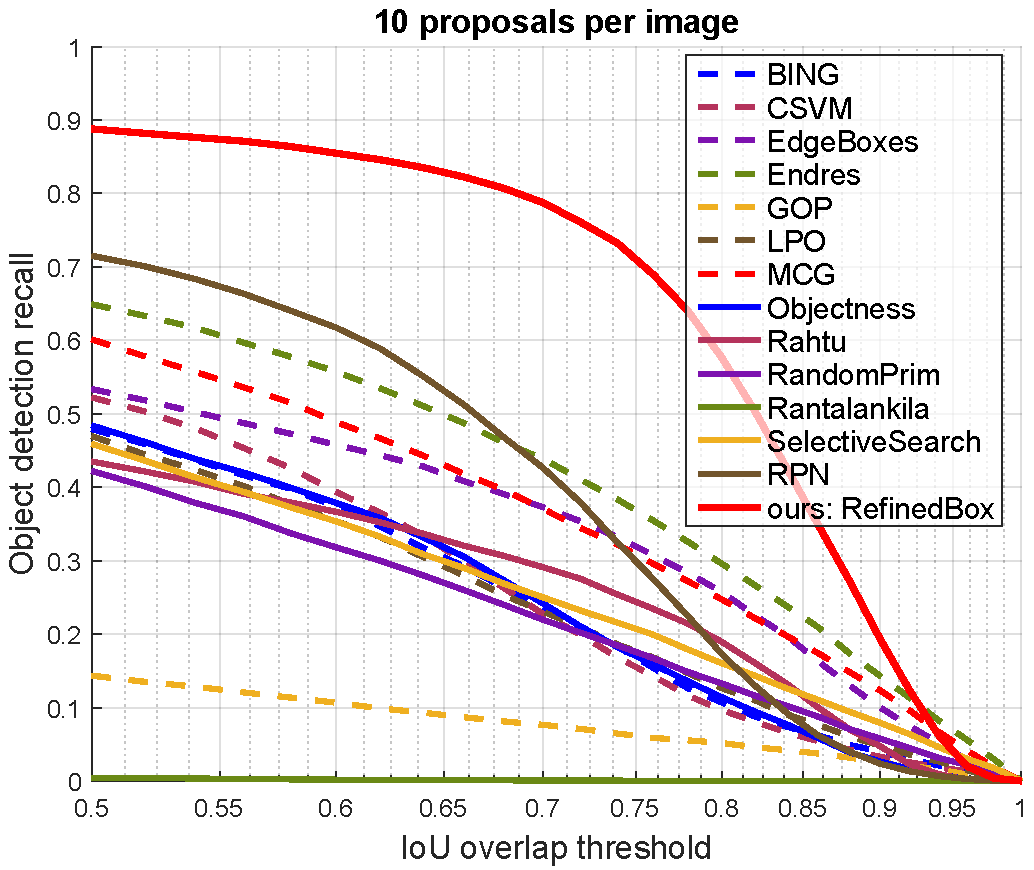
\includegraphics[width=.425\linewidth]{recall-threshold-10bb}} \hspace{.03\linewidth}
  \subfigure[]{
  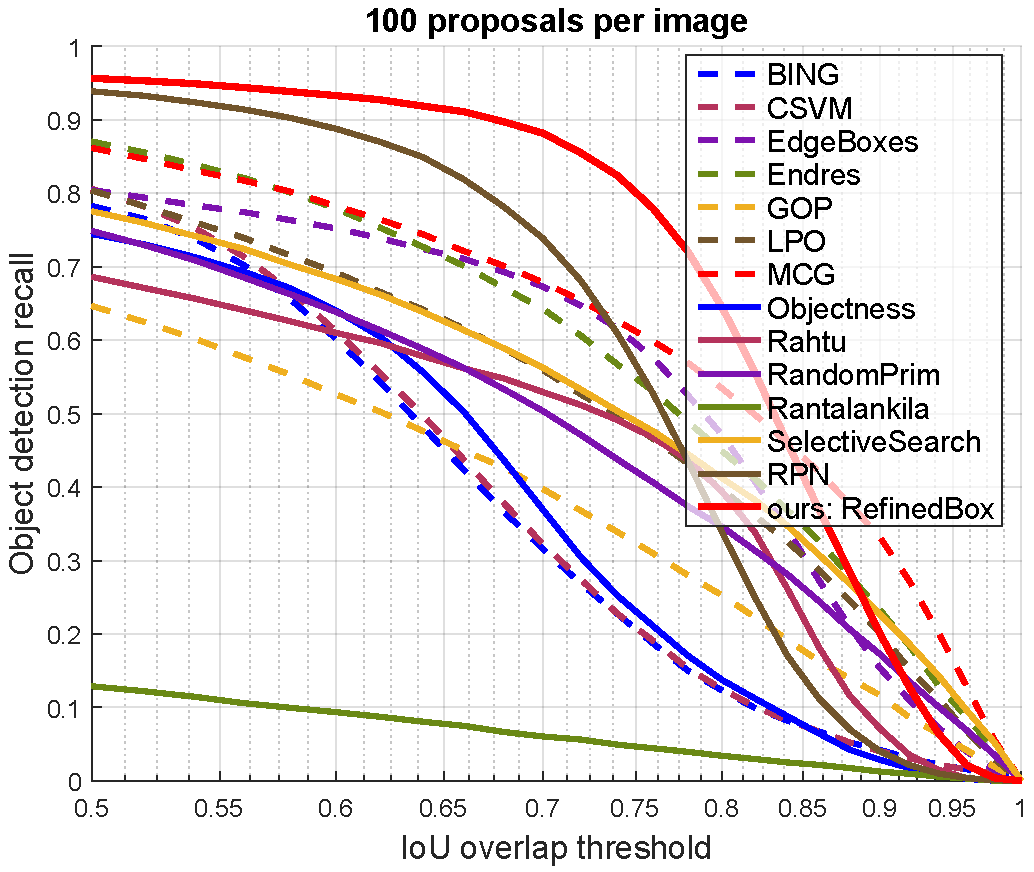
\includegraphics[width=.425\linewidth]{recall-threshold-100bb}} \\
  \subfigure[]{
  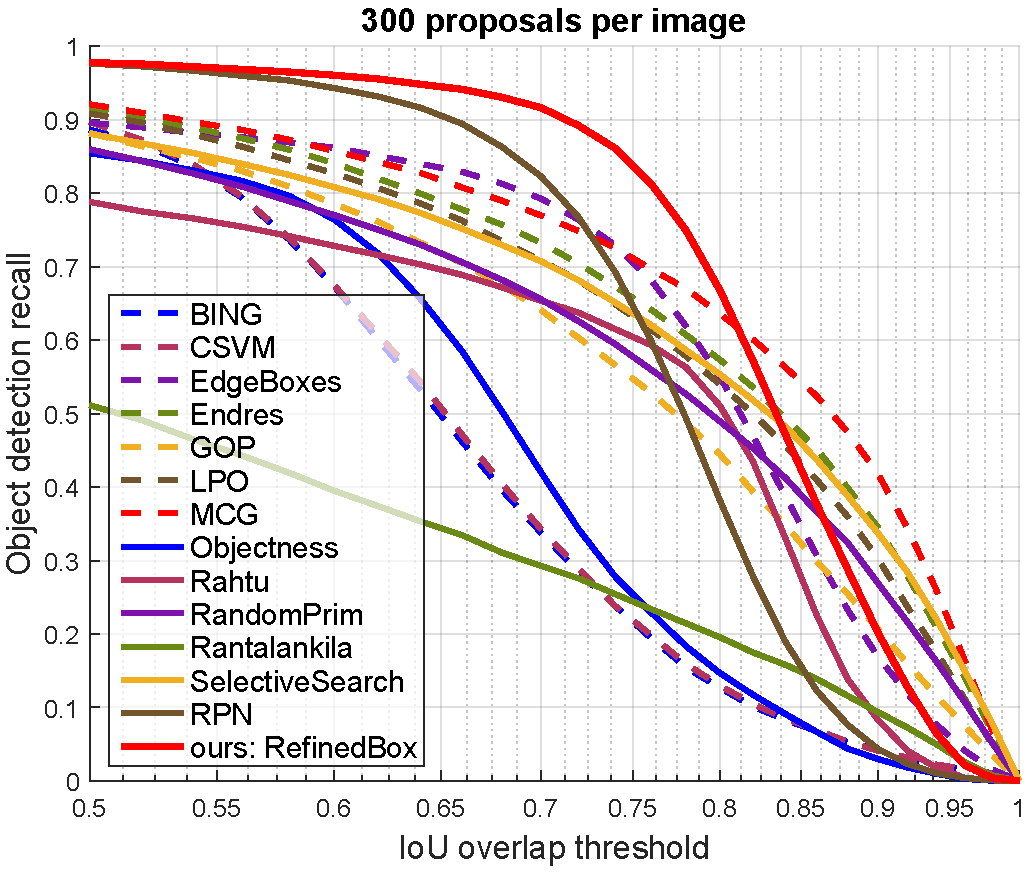
\includegraphics[width=.425\linewidth]{recall-threshold-300bb}} \hspace{.03\linewidth}
  \subfigure[]{
  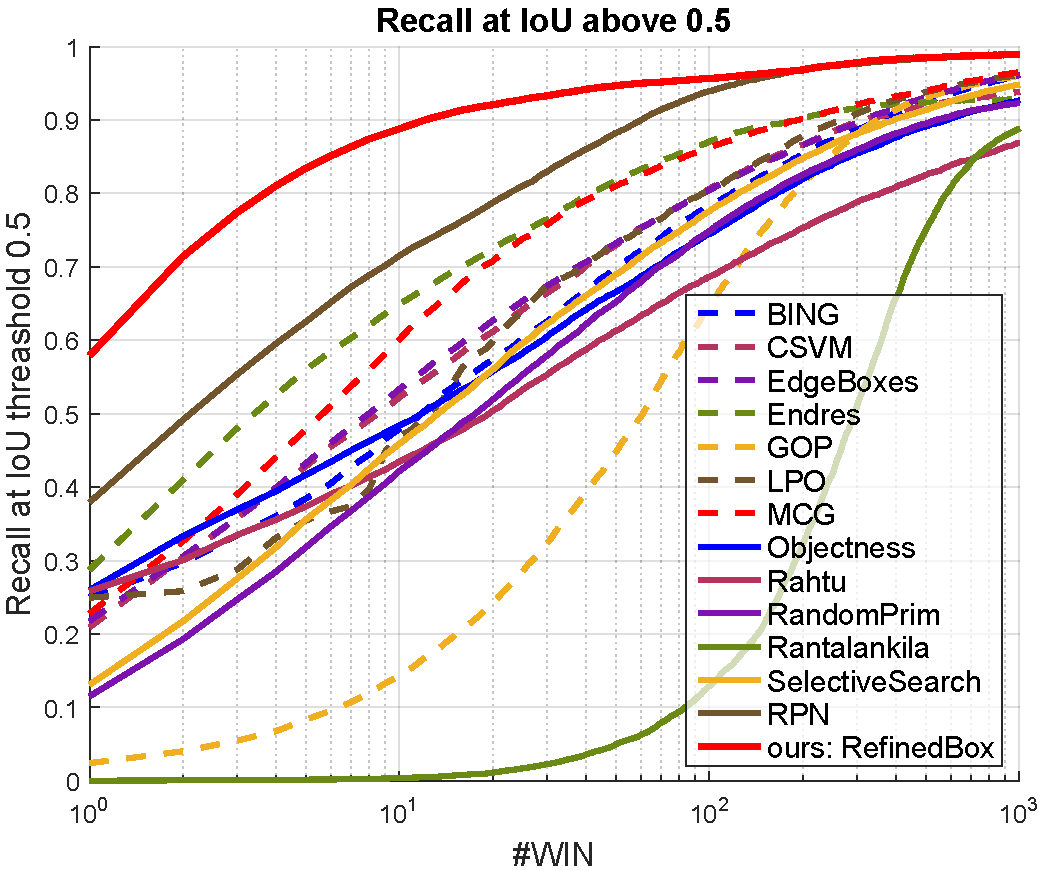
\includegraphics[width=.425\linewidth]{recall-proposals-0_5}} \\
  \subfigure[]{
  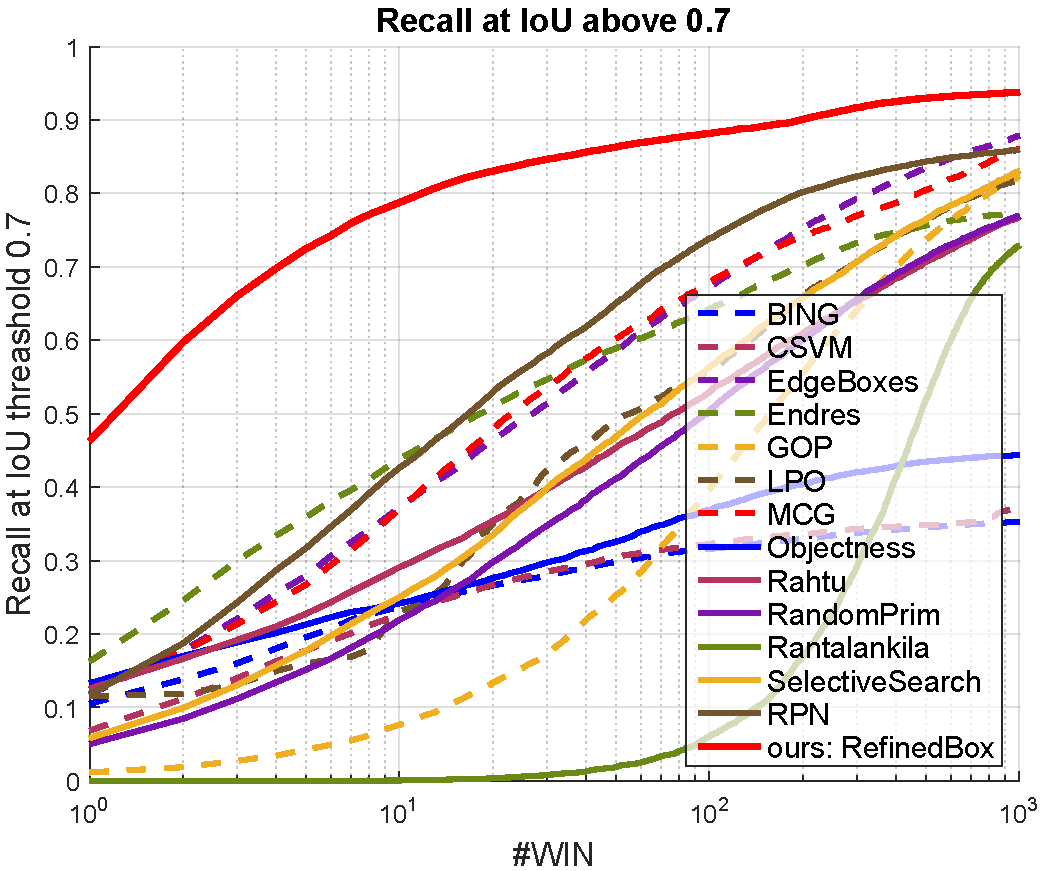
\includegraphics[width=.425\linewidth]{recall-proposals-0_7}} \hspace{.03\linewidth}
  \subfigure[]{
  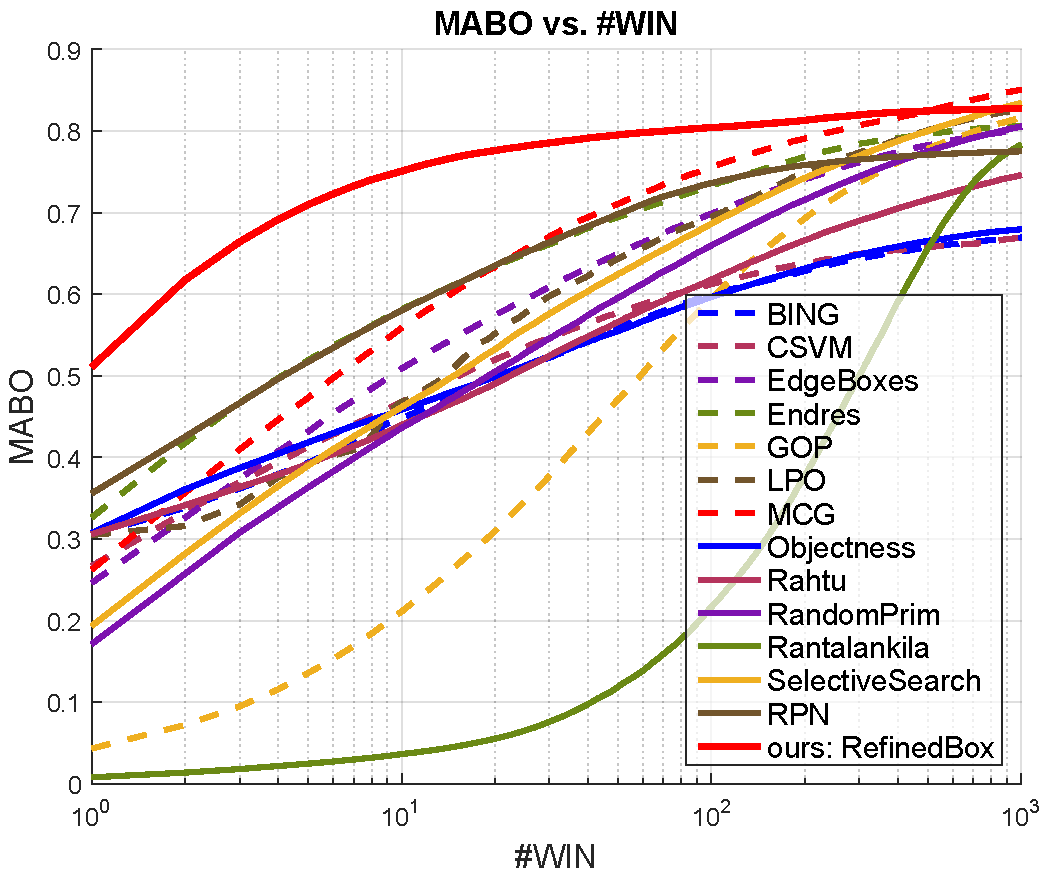
\includegraphics[width=.425\linewidth]{mabo-proposals}} \\
  \caption{The evaluation results on PASCAL VOC2007. (a)-(c) show object detection recall
  	\vs IoU overlap threshold, using 10, 100, 300 proposals per image respectively.
    (d)-(e) show object detection recall \vs the number of proposals (\#WIN) at IoU
    threshold 0.5 and 0.7 respectively. (f) shows MABO \vs the number of candidates
    using at most 1000 proposals per image.}
  \label{fig:voc-evaluation}
\end{figure*}


\subsection{Object Proposal Evaluation}
%
Here, we first compare our proposed RefinedBox with other proposal refinement
approaches such as DeepBox \cite{kuo2015deepbox} and MTSE \cite{chen2015improving}.
Then, we compare with some \sArt object proposal methods, including
Rahtu \cite{rahtu2011learning},
Objectness \cite{alexe2012measuring},
CSVM \cite{zhang2016object},
Selective Search \cite{uijlings2013selective},
RandomPrim \cite{manen2013prime},
Endres \cite{endres2014category},
Rantalankila \cite{rantalankila2014generating},
GoP \cite{krahenbuhl2014geodesic},
EdgeBoxes \cite{zitnick2014edge},
BING \cite{cheng2014bing},
MCG \cite{arbelaez2014multiscale},
LPO \cite{krahenbuhl2015learning},
RPN \cite{ren2015faster} and \etc.
% We take intersection-over-union (IoU) overlap scoring function as the
% measurement of the similarity between two bounding boxes.
% The IoU is the ration of intersection area of two bounding boxes and their union.
To evaluate the proposals, we adopt the metrics of object detection recall (DR)
and mean average best overlap (MABO).


\newcommand{\gEm}[1]{\underline{\bf #1}}
\newcommand{\tablefont}{\fontsize{8.2pt}{\baselineskip}\selectfont}

\begin{table}[!b]
	\vspace{-0.2in}
    \centering
    \setlength\tabcolsep{2.7pt}
    \caption{The evaluation results (\%) on the VOC2007 \textit{test} set.
    RefinedBox$^1$, RefinedBox$^2$, RefinedBox$^3$ and RefinedBox$^4$ mean
    RefinedBox with EdgeBoxes, MCG, SelectiveSearch and RPN respectively.}
    \label{tab:voc-evaluation}
    \begin{tabular*}{\linewidth}{c|c|c|c|c|c|c|c} \hline
        \multirow{2}*{} & \multicolumn{3}{c|}{DR (IoU=0.5)}
        				& \multicolumn{3}{c|}{DR (IoU=0.7)}
             			& \tablefont{MABO} \\ \cline{2-8}
        \diagbox{}{\#WIN} & 10 & 100 & 300  & 10 & 100 & 300 & 300  \\ \hline
        BING & 47.9 & 78.3 & 88.7 & 23.7 & 31.6 & 33.8 & 64.4 \\
        CSVM & 52.2 & 80.6 & 89.7 & 22.8 & 32.3 & 34.3 & 64.9 \\
        EdgeBoxes & 53.4 & 80.4 & 89.6 & 37.3 & 67.3 & 79.3 & 76.2 \\
        Endres & 64.9 & 87.1 & 91.6 & 43.9 & 64.3 & 73.3 & 78.4 \\
        GOP & 14.3 & 64.7 & 88.2 & 7.6 & 39.7 & 64.1 & 73.6 \\
        LPO & 47.0 & 80.4 & 90.9 & 23.1 & 56.0 & 70.9 & 77.4 \\
        MCG & 60.1 & 86.2 & 92.1 & 37.1 & 67.9 & 77.0 & 80.7 \\
        Objectness & 48.4 & 74.5 & 85.5 & 24.2 & 36.9 & 42.0 & 64.9 \\
        Rahtu & 43.5 & 68.6 & 78.8 & 29.1 & 52.9 & 65.4 & 69.0 \\
        RandomPrim & 42.2 & 74.9 & 86.0 & 22.0 & 50.4 & 65.6 & 74.4 \\
        Rantalankila & 0.4 & 12.9 & 51.1 &  0.1 & 6.0 & 29.3 & 50.0 \\
        SelectiveSearch & 45.9 & 77.6 & 88.1 & 25.0 & 56.3 & 70.7 & 77.0 \\
        RPN & 71.5 & 93.9 & 97.7 & 42.6 & 73.9 & 82.3 & 76.5 \\ \hline
        RefinedBox$^1$ & \gEm{88.8} & \gEm{95.7} & \gEm{97.8} & \gEm{78.8}
        	& \gEm{88.2} & \gEm{91.7} & \gEm{82.0} \\
        RefinedBox$^2$ & 88.3 & 94.9 & 97.4 & 78.1 & 85.0 & 88.1 & 81.4 \\
        RefinedBox$^3$ & 87.9 & 93.5 & 95.6 &  \gEm{78.8} & 85.5 & 88.2 & 80.7 \\
        RefinedBox$^4$ & \gEm{88.8} & 95.5 & 97.2 & 76.5 & 85.9 & 89.6
        	& 79.9 \\ \hline
    \end{tabular*}
\end{table}


The comparison between different proposal refinement approaches is shown
in \figref{fig:refine-evaluation}.
We choose Edge Boxes \cite{zitnick2014edge} to produce the initial proposals
which are inputted into these refinement algorithms, but we change the default
parameter of non-maximum suppression from 0.75 to 0.9 in order to obtain more boxes.
% The method of EdgeBoxes-default uses the default parameters of EdgeBoxes,
% while the EdgeBoxes-NMS-0.9 changes the NMS threshold to 0.9.
We find that our method achieves much higher object detection recall than other
competitors at both IoU thresholds 0.5 and 0.7.
The gap between our RefinedBox and other competitors is very large.
Using only one proposal per image, RefinedBox achieves a detection recall of
57.9\% and 46.3\% at IoU 0.5 and IoU 0.7, respectively.
In addition, RefinedBox can share the convolutional layer with subsequent object
detection and the additional layers of RefinedBox are computationally lightweight,
so RefinedBox is an efficient detection framework.
In fact, the total time consumption of RefinedBox and subsequent object detection
is similar to the Faster R-CNN \cite{ren2015faster} at about 0.13 second per image.
DeepBox builds a separate network to re-rank boxes,
while MTSE segments an image first and then uses superpixels to refine boxes;
however, the image segmentation step is a time-consuming operation.
Thus, RefinedBox is more suitable to be used in object detection.


Extensive comparisons with other object proposal generation methods
are shown in \figref{fig:voc-evaluation}.
RefinedBox also uses EdgeBoxes as input,
and we apply the default parameters for the evaluation of EdgeBoxes.
Our method achieves the \sArt performance across all cases.
RPN has recently become popular for object detection,
but our proposed RefinedBox is much more accurate than it.
The object detection recall of RefinedBox with only 10 proposals per image
is similar to RPN using 100 proposals per image.
The improvement from RPN to RefinedBox demonstrates the effectiveness of our method.
We also observe that the detection recall of RPN drops sharply for high IoU
thresholds.
Although RefinedBox also suffers a drop for high IoU thresholds,
it always performs better than RPN and EdgeBoxes.
We believe that this is due to the initial input boxes
and that this problem can be overcome if some other proposal generation methods are used.
For object detection recall \vs the number of proposals at IoU 0.7,
the performance improvements between RefinedBox and other competitors are also very large.
The higher detection recall and fewer proposals will benefit the subsequent
object detection a lot.


To quantify these plots, we list the corresponding numbers
in \tabref{tab:voc-evaluation}.
RefinedBox achieves much better performance than various initial
input methods.
With EdgeBoxes and an IoU threshold of 0.5, the detection recall of RefinedBox
is 17.3\%, 1.8\%, and 0.1\% higher than the second place method (RPN) when
using 10, 100, and 300 proposals per image, respectively.
At an IoU threshold of 0.7, the detection recall of RefinedBox with EdgeBoxes
is 36.2\%, 14.3\% and 9.4\% higher than RPN when 10, 100 and 300 proposals
are used per image respectively.
Using 300 proposals per image, the MABO of RefinedBox is 1.3\% higher than
MCG, which achieves the second place on this metric.
We also notice that RPN is much better than other competitors except RefinedBox.
This is the key reason why Faster R-CNN can achieve better detection performance
than Fast R-CNN.
% EdgeBoxes and MCG achieve the \sArt performance among non-deep learning
% based methods.
% That is why we choose EdgeBoxes as the input of RefinedBox.


\begin{table*}[!htbp]
    \centering
    \setlength\tabcolsep{1.65pt}
    \caption{Detection average precision (\%) using Fast R-CNN on the VOC2007
    	test set. Note that the RPN below means Faster R-CNN. RefinedBox$^1$,
        RefinedBox$^2$, RefinedBox$^3$ and RefinedBox$^4$ mean RefinedBox
        with EdgeBoxes, MCG, SelectiveSearch and RPN respectively.}
    \label{tab:voc-detection}
    \begin{tabular*}{\textwidth}{c|cccccccccccccccccccc|c} \hline
        Methods & aer. & bic. & bird & boat & bot. & bus & car & cat & cha.
        & cow & din. & dog & hor. & mot. & per. & pot. & she. & sofa & tra.
        & tv & mAP\\ \hline
        %
        BING&65.0&68.6&61.8&46.8&42.2&72.1&71.4&77.7&31.4&69.7
            &56.3&74.0&75.7&66.3&65.4&27.1&62.1&60.6&68.7&60.0&61.2\\
        %
        CSVM&68.0&71.3&60.3&44.1&33.7&73.0&69.1&77.1&28.7&68.1
            &58.7&71.5&78.3&69.5&60.7&25.6&57.4&61.4&72.5&55.7&60.2\\
        %
        EdgeBoxes&\gEm{73.4}&78.1&68.4&55.7&39.2&79.5&76.8&81.0&41.7&73.7
        		 &65.6&82.8&82.6&76.2&68.1&34.8&66.2&70.1&77.1&58.9&67.5\\
        %
        Endres&63.3&75.0&63.4&43.0&31.2&77.2&70.5&78.1&32.8&66.8
              &67.6&75.3&78.7&70.9&61.1&28.0&61.6&66.3&75.9&61.3&62.4\\
        %
        GOP&67.2&76.3&65.7&51.5&32.4&78.4&78.6&81.1&40.7&74.1
           &64.2&78.7&80.5&74.3&67.3&30.7&65.4&\gEm{70.6}&76.5&66.1&66.0\\
        %
        LPO&67.4&76.9&\gEm{68.8}&52.1&30.4&81.3&75.0&79.9&37.9&73.9
           &67.6&76.4&80.3&70.1&66.1&33.5&65.0&68.0&76.4&63.9&65.6\\
        %
        MCG&69.8&77.2&67.2&51.8&42.5&80.0&76.8&78.6&43.9&71.4
           &68.1&77.1&81.5&70.9&67.8&33.0&65.5&68.2&77.1&64.8&66.7\\
        %
        Objectness&64.7&73.5&60.4&40.1&34.8&72.7&69.5&76.8&31.5&67.4
        		  &59.0&77.7&79.1&71.4&60.8&30.5&54.6&62.0&73.5&57.5&60.9\\
        %
        Rahtu&69.2&68.6&59.1&53.8&23.1&78.4&67.2&79.9&26.9&66.6
        	 &68.5&76.7&79.7&70.3&58.0&26.9&57.1&64.2&77.2&60.5&61.6\\
        %
        RandomPrim&69.8&78.4&61.5&52.6&25.3&76.0&69.3&78.3&39.2&67.5&\gEm{69.8}
        	      &76.2&\gEm{82.7}&69.5&58.8&27.6&53.7&67.5&76.3&58.5&62.9\\
        %
        Rantalankila&68.0&67.7&63.1&42.3&21.5&71.5&64.5&78.7&29.8&69.2
        			&67.6&74.3&77.1&66.9&54.7&25.2&60.6&63.8&75.9&59.9&60.1\\
        %
        SelectiveSearch&72.9&78.3&66.0&54.3&34.7&81.3&76.8&83.3&41.5&74.5&66.4
        			   &79.8&82.2&76.2&65.5&35.2&65.6&70.1&\gEm{77.4}&65.9&67.4\\
        %
        RPN&67.5&78.5&67.3&51.9&51.5&76.2&79.8&84.4&50.2&74.3&66.9&\gEm{83.2}
		   &80.0&73.9&76.5&37.1&\gEm{69.4}&65.7&76.5&74.2&69.2 \\ \hline
        %
        RefinedBox$^1$&70.0&79.7&66.4&58.8&\gEm{58.0}&78.3&80.0
        	&\gEm{86.4}&52.2&73.7&\gEm{69.8}&81.4&80.6&75.9&77.6
            &\gEm{46.5}&68.1&67.8&76.7&73.1&\gEm{71.1} \\
        RefinedBox$^2$&68.6&\gEm{80.1}&67.5&55.0&55.5&79.2&79.4&79.7&51.6&75.3&
        65.8&76.7&80.7&76.9&77.4&41.3&68.5&69.8&\gEm{77.4}&\gEm{74.8}&70.1\\
        RefinedBox$^3$&68.1&78.2&67.7&\gEm{59.5}&56.4&83.4&\gEm{80.3}&79.4&\gEm{52.9}
        &75.1&\gEm{69.8}&77.2&80.4&76.2&\gEm{78.2}&42.0&69.0&69.4&76.1&73.7&70.7\\
        RefinedBox$^4$&68.6&79.4&68.2&55.6&56.1&\gEm{84.0}&80.2&84.1&52.8&\gEm{75.5}
    	&\gEm{69.8}&77.8&80.6&\gEm{77.1}&78.1&43.9&67.3&65.6&75.8&72.8&70.7\\ \hline
    \end{tabular*}
\end{table*}


\begin{figure*}[!t]
  \centering
  \newcommand{\AddImg}[1]{\includegraphics[height=.143\linewidth]{ilu/#1.png}}
  \AddImg{000038}\hfill \AddImg{000062}\hfill \AddImg{000069}\hfill
  \AddImg{000071}\hfill \AddImg{000076}
  \\ \vspace{.03in}
  \renewcommand{\AddImg}[1]{\includegraphics[height=.20\linewidth]{ilu/#1.png}}
  \AddImg{000010}\hfill \AddImg{003041}\hfill \AddImg{003572}\hfill
  \AddImg{003592}\hfill \AddImg{003854}\hfill \AddImg{003976}\hfill
  \AddImg{006640}
  \\ \vspace{.03in}
  \renewcommand{\AddImg}[1]{\includegraphics[height=.143\linewidth]{ilu/#1.png}}
  \AddImg{000124}\hfill \AddImg{000319}\hfill \AddImg{000570}\hfill
  \AddImg{003647}\hfill \AddImg{003910}
  \\
  \caption{Some detection samples of our method. All images are from VOC2007
  		\textit{test} set.}
  \label{fig:visual}
  \vspace{-0.008in}
\end{figure*}



\subsection{Object Detection}
%
Since object proposal generation aims to provide proposals
for consequent object detection, the quality of proposals
needs to be tested in object detection.
We therefore feed the proposals produced by the aforementioned
methods into a well-known region-based object detection framework,
Fast R-CNN \cite{girshick2015fast}.
We test RefinedBox using the joint training method described above.
For RPN, we simply test Faster R-CNN \cite{ren2015faster}.
For other bottom-up methods, we follow the settings
in \cite{zhang2017sequential}.
We use the top 1000 proposals per image to retrain the Fast R-CNN
network and then test them.
All of these methods are trained on the VOC2007 \textit{trainval} set
and tested on the \textit{test} set.


The results are listed in \tabref{tab:voc-detection}.
% In terms of mean average precision (mAP), RefinedBox is 1.9\% higher
% than RPN (Faster R-CNN) and 3.6\% higher than original EdgeBoxes.
% RefinedBox achieves the best average precision (AP) on 9 categories among the
% 20 categories of VOC2007 dataset.
% The overall detection performance of some proposal algorithms is quite close to
% each other, \ie EdgeBoxes, GOP, LPO, MCG and SelectiveSearch.
% BING, CSVM, Endres, Objectness, Rahtu, RandomPrim and Rantalankila
% perform worse.
In terms of mAP, RefinedBox is 3.6\%, 3.4\%,
3.3\% and 1.5\% higher than the original proposal methods, \ie
EdgeBoxes, MCG, SelectiveSearch and RPN, respectively.
The best performance of RefinedBox is 1.9\% higher than Faster R-CNN.
These evaluation results demonstrate the effectiveness of RefinedBox
in object detection.
Since RefinedBox can be embedded into a detection network as a
computationally lightweight branch, it has the potential to significantly
improve object detection.
We show some detection examples produced by RefinedBox in \figref{fig:visual}.



%%%%%%%%%%%%%%%%%%%%%%%%%%%%%%%%%%%%%%%%%%%%%%%%%%%%%%%%%%%%%%%%%%%%%%%%%%%%%%%
\section{Conclusion}
%
In this paper, we present a proposal refinement
method using re-ranking and box regression.
Our proposed RefinedBox can share the convolutional
layers with subsequent object detection,
and its unique layers are computationally lightweight.
Extensive experiments demonstrate that RefinedBox can generate
high-quality proposals and that these proposals can lead to higher object
detection performance than the well-known algorithm Faster R-CNN.
RefinedBox's effectiveness and efficiency means that it has the
potential to be embedded in other object detection networks
such as \cite{ren2015faster,lin2016feature,kong2017ron}.
RefinedBox can also be applied to reduce the number of proposals
for other tasks that need fewer but high-quality proposals as input
such as \cite{wei2016hcp,paisitkriangkrai2016pedestrian,wu2015deep}.
To promote the development of this field, the code of this paper
will be published as soon as the paper is accepted.



\bibliographystyle{aaai}
\bibliography{RefinedBox}

\end{document} 